\documentclass[ignorenonframetext,]{beamer}
\setbeamertemplate{caption}[numbered]
\setbeamertemplate{caption label separator}{:}
\setbeamercolor{caption name}{fg=normal text.fg}
\usepackage{amssymb,amsmath}
\usepackage{ifxetex,ifluatex}
\usepackage{fixltx2e} % provides \textsubscript
\usepackage{lmodern}
\ifxetex
  \usepackage{fontspec,xltxtra,xunicode}
  \defaultfontfeatures{Mapping=tex-text,Scale=MatchLowercase}
  \newcommand{\euro}{€}
\else
  \ifluatex
    \usepackage{fontspec}
    \defaultfontfeatures{Mapping=tex-text,Scale=MatchLowercase}
    \newcommand{\euro}{€}
  \else
    \usepackage[T1]{fontenc}
    \usepackage[utf8]{inputenc}
      \fi
\fi
% use upquote if available, for straight quotes in Verbatim environments
\IfFileExists{upquote.sty}{\usepackage{upquote}}{}
% use microtype if available
\IfFileExists{microtype.sty}{\usepackage{microtype}}{}
\usepackage{color}
\usepackage{fancyvrb}
\newcommand{\VerbBar}{|}
\newcommand{\VERB}{\Verb[commandchars=\\\{\}]}
\DefineVerbatimEnvironment{Highlighting}{Verbatim}{commandchars=\\\{\},fontsize=\small}
% Add ',fontsize=\small' for more characters per line
\usepackage{framed}
\definecolor{shadecolor}{RGB}{248,248,248}
\newenvironment{Shaded}{\begin{snugshade}}{\end{snugshade}}
\newcommand{\KeywordTok}[1]{\textcolor[rgb]{0.13,0.29,0.53}{\textbf{{#1}}}}
\newcommand{\DataTypeTok}[1]{\textcolor[rgb]{0.13,0.29,0.53}{{#1}}}
\newcommand{\DecValTok}[1]{\textcolor[rgb]{0.00,0.00,0.81}{{#1}}}
\newcommand{\BaseNTok}[1]{\textcolor[rgb]{0.00,0.00,0.81}{{#1}}}
\newcommand{\FloatTok}[1]{\textcolor[rgb]{0.00,0.00,0.81}{{#1}}}
\newcommand{\CharTok}[1]{\textcolor[rgb]{0.31,0.60,0.02}{{#1}}}
\newcommand{\StringTok}[1]{\textcolor[rgb]{0.31,0.60,0.02}{{#1}}}
\newcommand{\CommentTok}[1]{\textcolor[rgb]{0.56,0.35,0.01}{\textit{{#1}}}}
\newcommand{\OtherTok}[1]{\textcolor[rgb]{0.56,0.35,0.01}{{#1}}}
\newcommand{\AlertTok}[1]{\textcolor[rgb]{0.94,0.16,0.16}{{#1}}}
\newcommand{\FunctionTok}[1]{\textcolor[rgb]{0.00,0.00,0.00}{{#1}}}
\newcommand{\RegionMarkerTok}[1]{{#1}}
\newcommand{\ErrorTok}[1]{\textbf{{#1}}}
\newcommand{\NormalTok}[1]{{#1}}
\usepackage{longtable,booktabs}
\usepackage{caption}
% These lines are needed to make table captions work with longtable:
\makeatletter
\def\fnum@table{\tablename~\thetable}
\makeatother
\usepackage{graphicx}
\makeatletter
\def\maxwidth{\ifdim\Gin@nat@width>\linewidth\linewidth\else\Gin@nat@width\fi}
\def\maxheight{\ifdim\Gin@nat@height>\textheight0.8\textheight\else\Gin@nat@height\fi}
\makeatother
% Scale images if necessary, so that they will not overflow the page
% margins by default, and it is still possible to overwrite the defaults
% using explicit options in \includegraphics[width, height, ...]{}
\setkeys{Gin}{width=\maxwidth,height=\maxheight,keepaspectratio}

% Comment these out if you don't want a slide with just the
% part/section/subsection/subsubsection title:
\AtBeginPart{
  \let\insertpartnumber\relax
  \let\partname\relax
  \frame{\partpage}
}
\AtBeginSection{
  \let\insertsectionnumber\relax
  \let\sectionname\relax
  \frame{\sectionpage}
}
\AtBeginSubsection{
  \let\insertsubsectionnumber\relax
  \let\subsectionname\relax
  \frame{\subsectionpage}
}

\setlength{\parindent}{0pt}
\setlength{\parskip}{6pt plus 2pt minus 1pt}
\setlength{\emergencystretch}{3em}  % prevent overfull lines
\setcounter{secnumdepth}{0}

\title{Regression}
\author{Mark Hagemann}
\date{March 5, 2015}

\begin{document}
\frame{\titlepage}

\begin{frame}[fragile]

\begin{Verbatim}[fontsize=\small]
## 
## Attaching package: 'dplyr'
## 
## The following object is masked from 'package:stats':
## 
##     filter
## 
## The following objects are masked from 'package:base':
## 
##     intersect, setdiff, setequal, union
\end{Verbatim}

\end{frame}

\begin{frame}{Outline}

\begin{itemize}[<+->]
\itemsep1pt\parskip0pt\parsep0pt
\item
  What is a regression model and what's it good for?

  \begin{itemize}[<+->]
  \itemsep1pt\parskip0pt\parsep0pt
  \item
    Explanation
  \item
    Quantifying relationships
  \item
    Prediction
  \end{itemize}
\item
  Limitations

  \begin{itemize}[<+->]
  \itemsep1pt\parskip0pt\parsep0pt
  \item
    Assumptions (linearity, i.i.d., etc.)
  \item
    Predicting is hard!
  \end{itemize}
\end{itemize}

\end{frame}

\begin{frame}{Approach}

\begin{itemize}[<+->]
\itemsep1pt\parskip0pt\parsep0pt
\item
  Look at your data
\item
  build model(s)
\item
  Check assumptions
\item
  select model
\item
  Use model
\end{itemize}

\end{frame}

\begin{frame}{Math background}

\end{frame}

\begin{frame}{Linear functions}

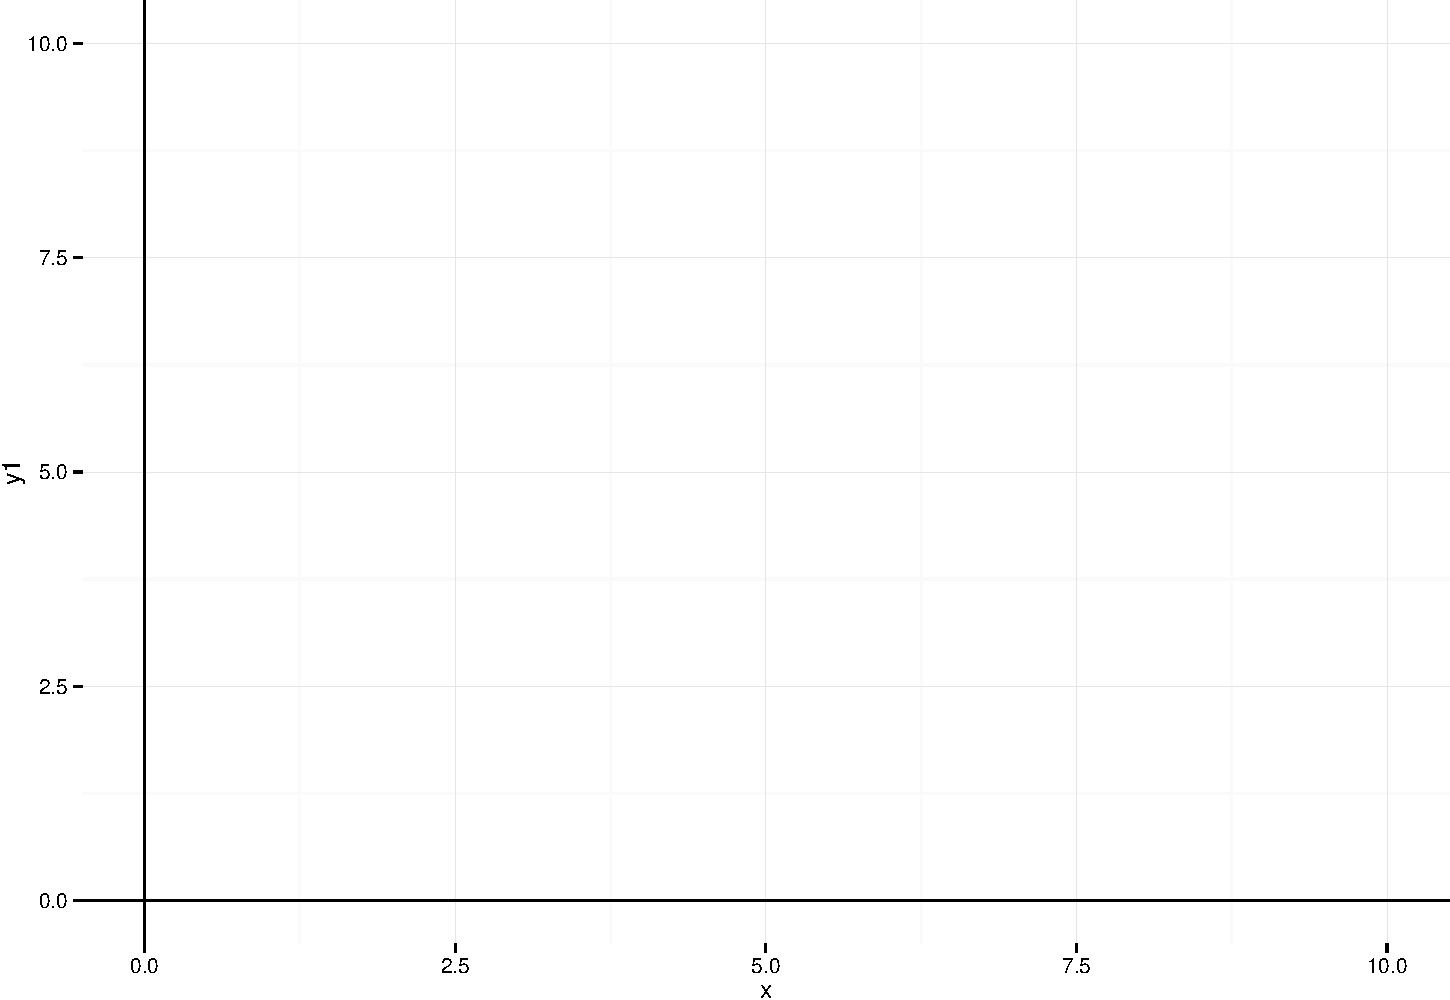
\includegraphics{Regression_files/figure-beamer/linfun-1.pdf}

\end{frame}

\begin{frame}{Linear functions}

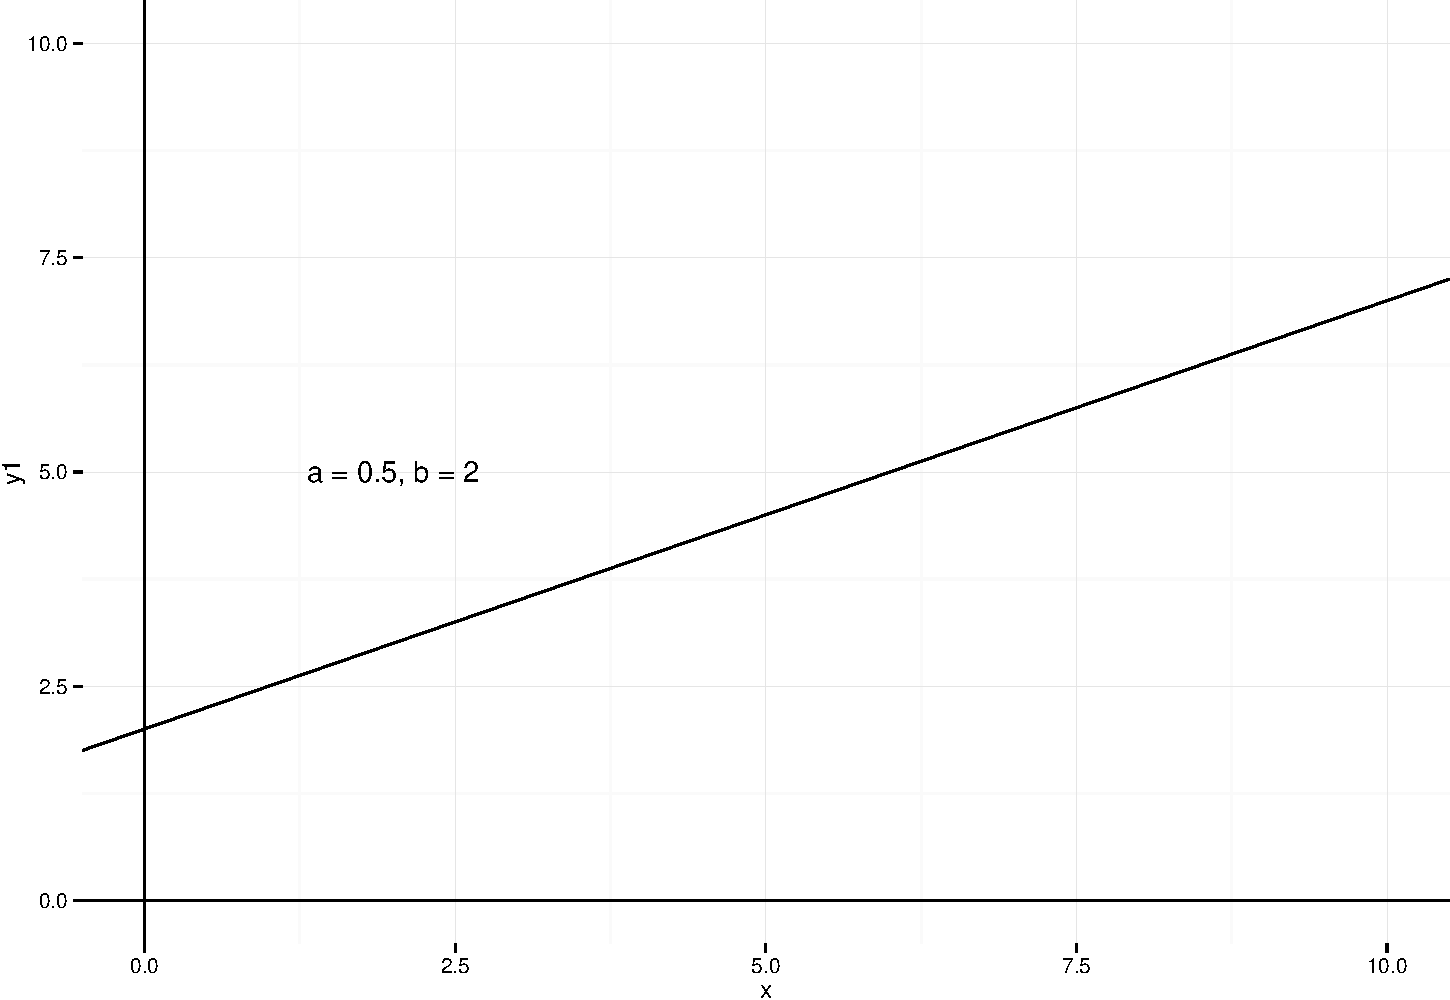
\includegraphics{Regression_files/figure-beamer/unnamed-chunk-1-1.pdf}

\begin{itemize}[<+->]
\itemsep1pt\parskip0pt\parsep0pt
\item
  \(y = a \times x + b\)
\end{itemize}

\end{frame}

\begin{frame}{Some (perfectly linear) data}

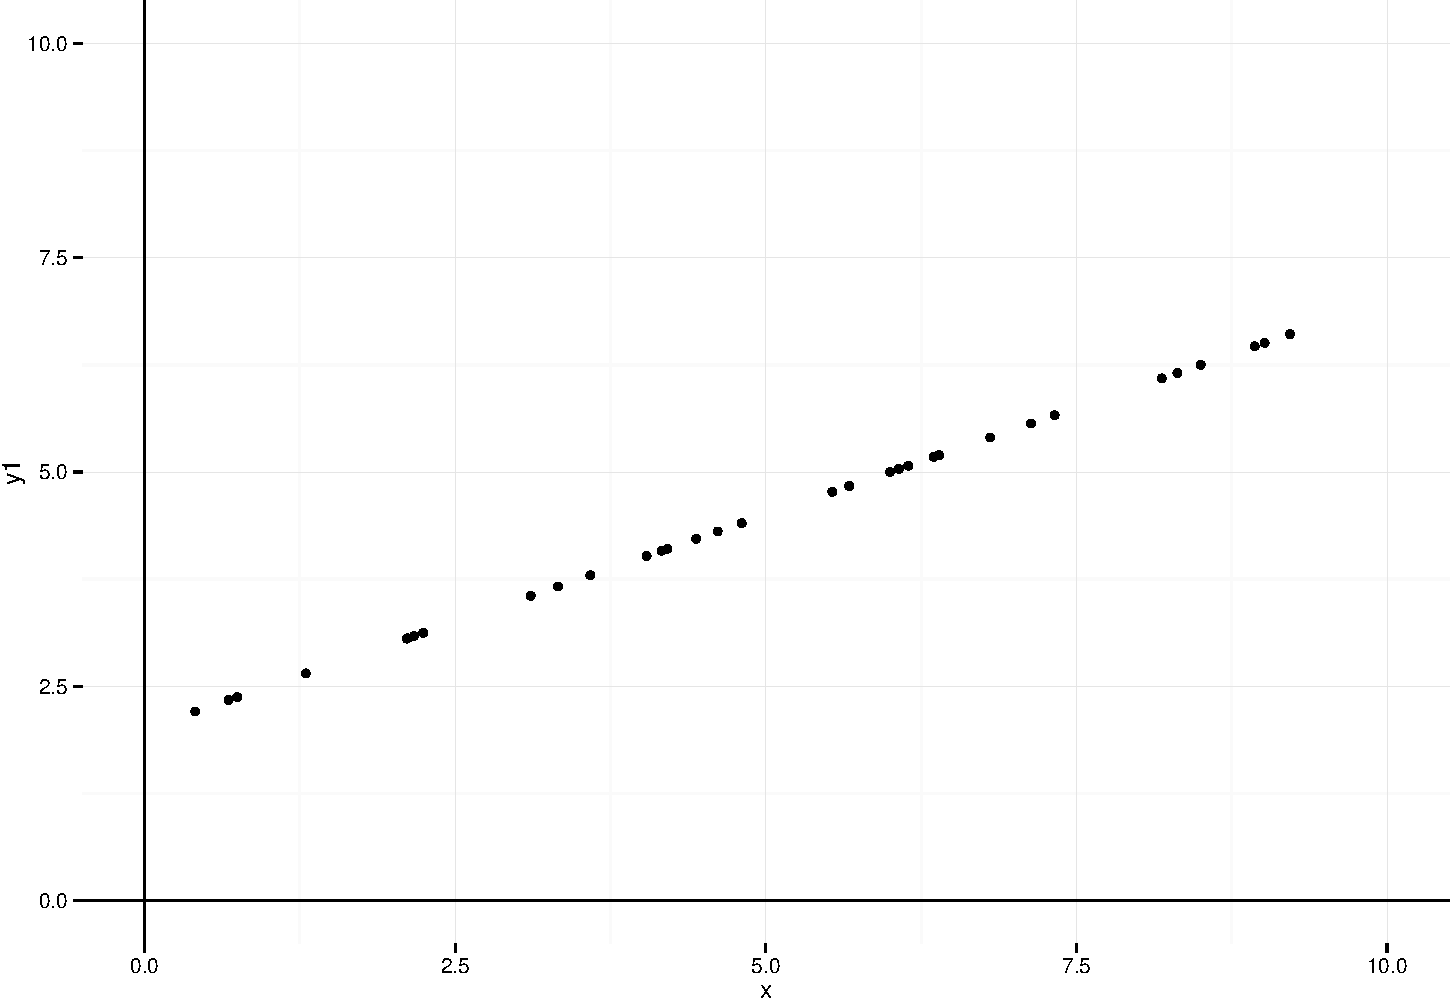
\includegraphics{Regression_files/figure-beamer/unnamed-chunk-2-1.pdf}

\end{frame}

\begin{frame}{A (perfect) linear regression line}

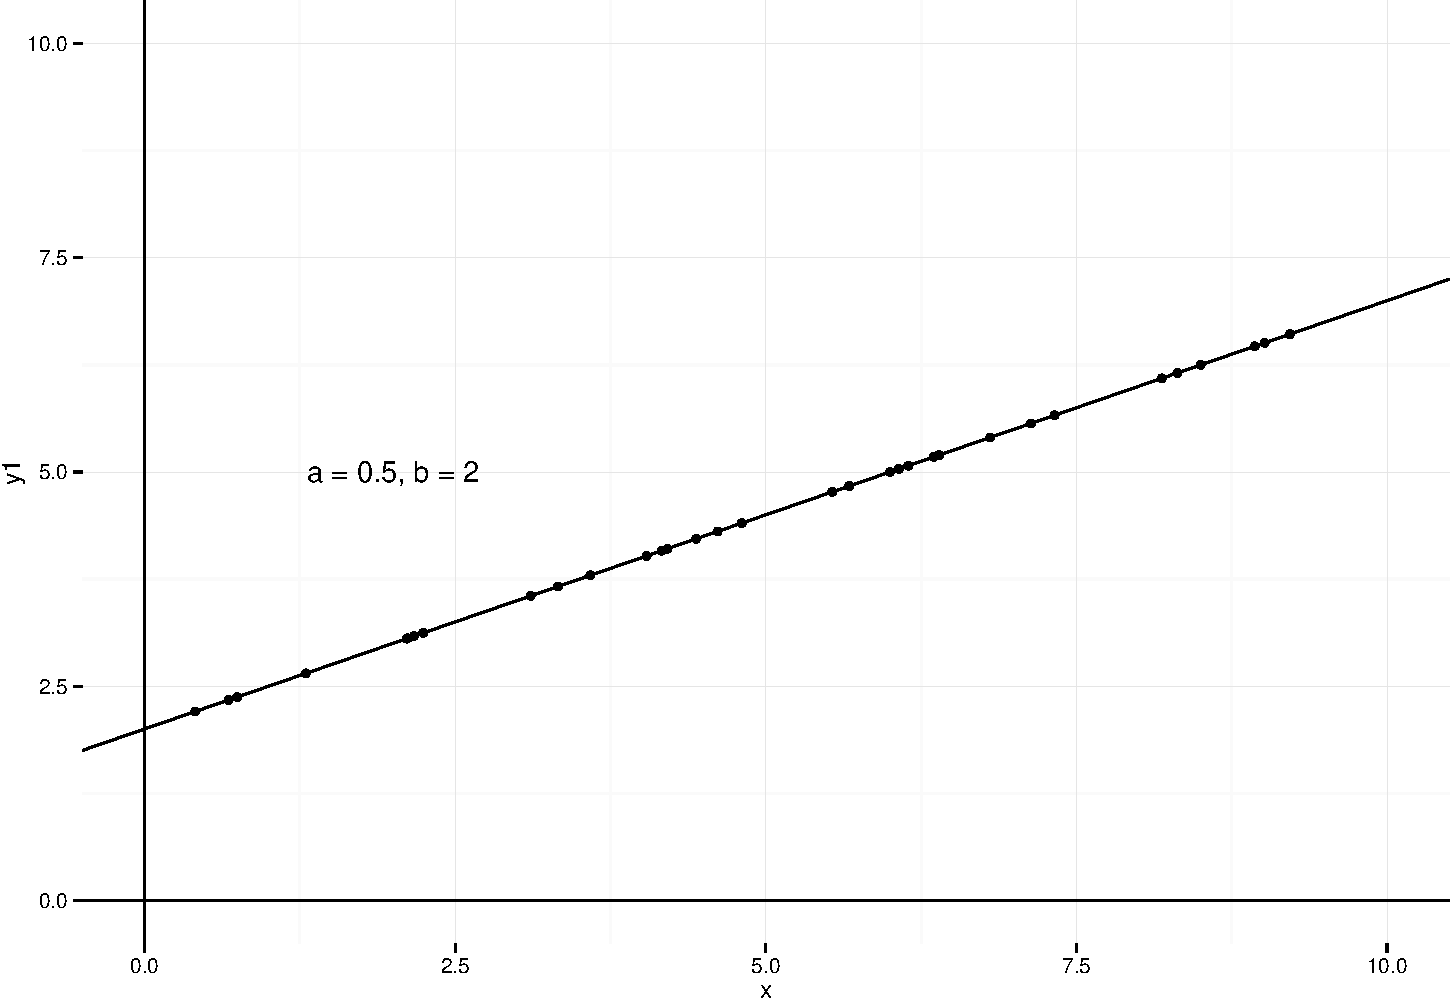
\includegraphics{Regression_files/figure-beamer/unnamed-chunk-3-1.pdf}

\end{frame}

\begin{frame}{More realistic case}

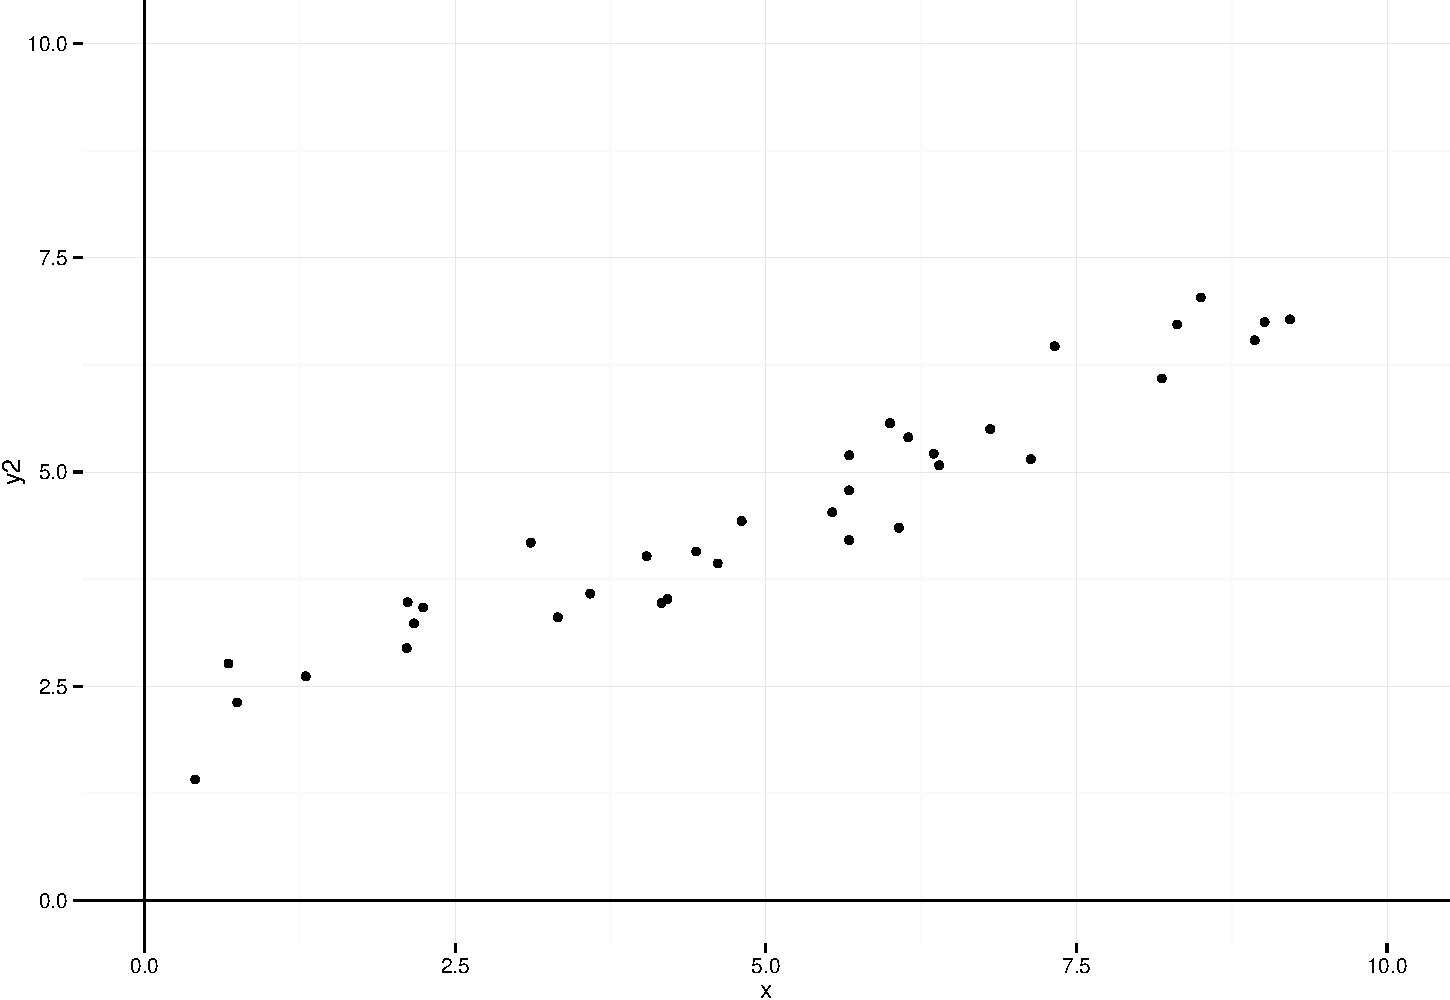
\includegraphics{Regression_files/figure-beamer/unnamed-chunk-4-1.pdf}

\begin{block}{In reality, we start with the (noisy) data, and we seek
the underlying function}

\end{block}

\end{frame}

\begin{frame}{Fit a line}

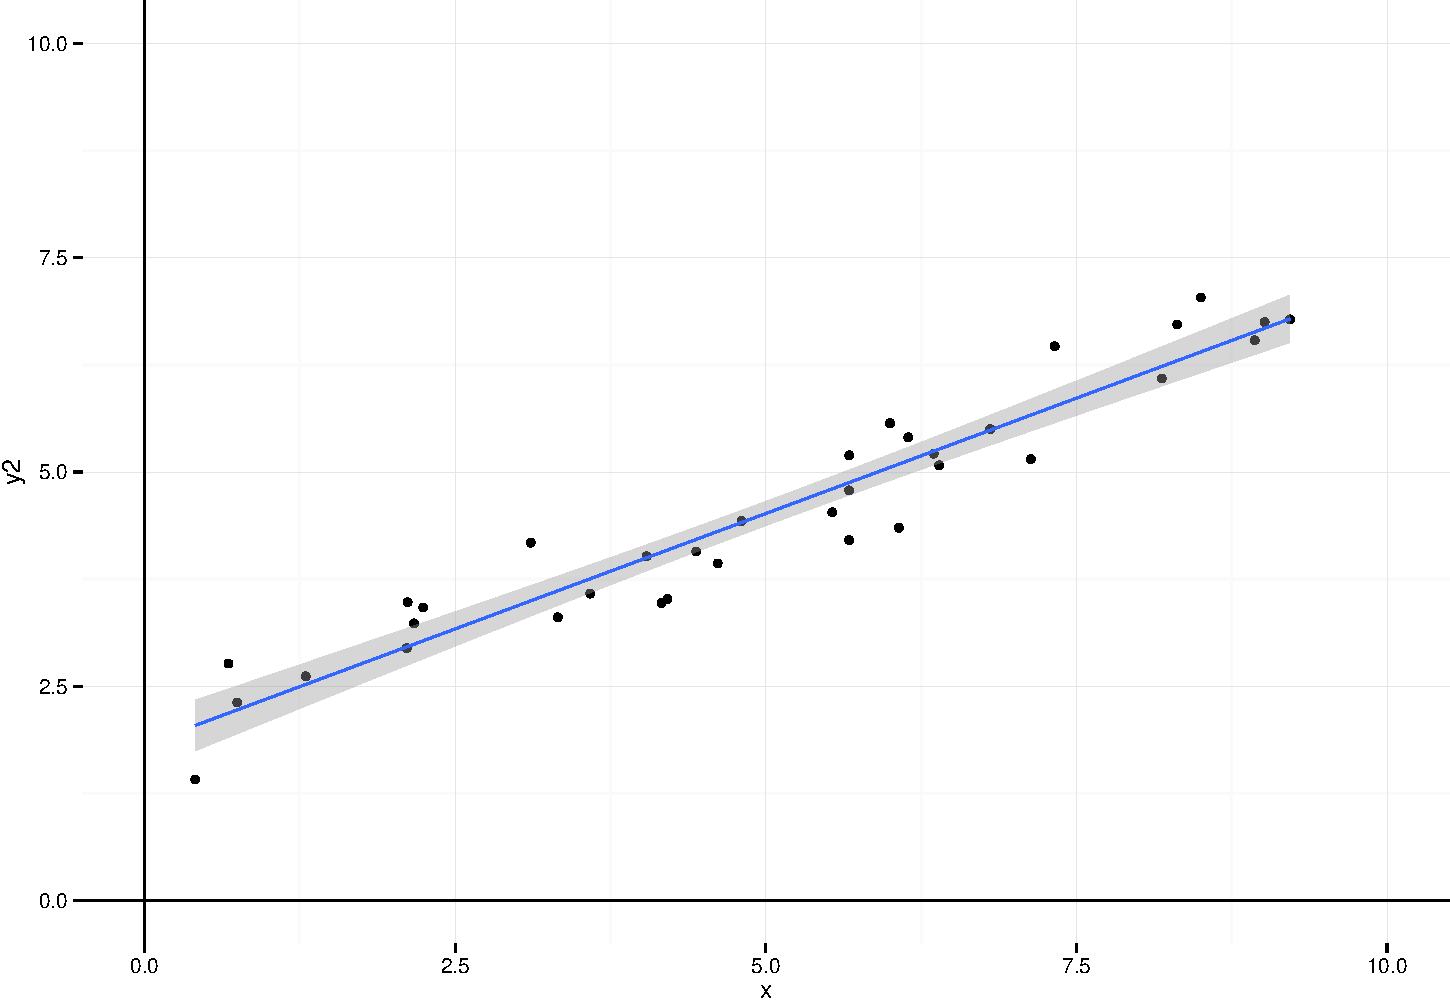
\includegraphics{Regression_files/figure-beamer/unnamed-chunk-5-1.pdf}

\end{frame}

\begin{frame}{Compare to ``actual'' function}

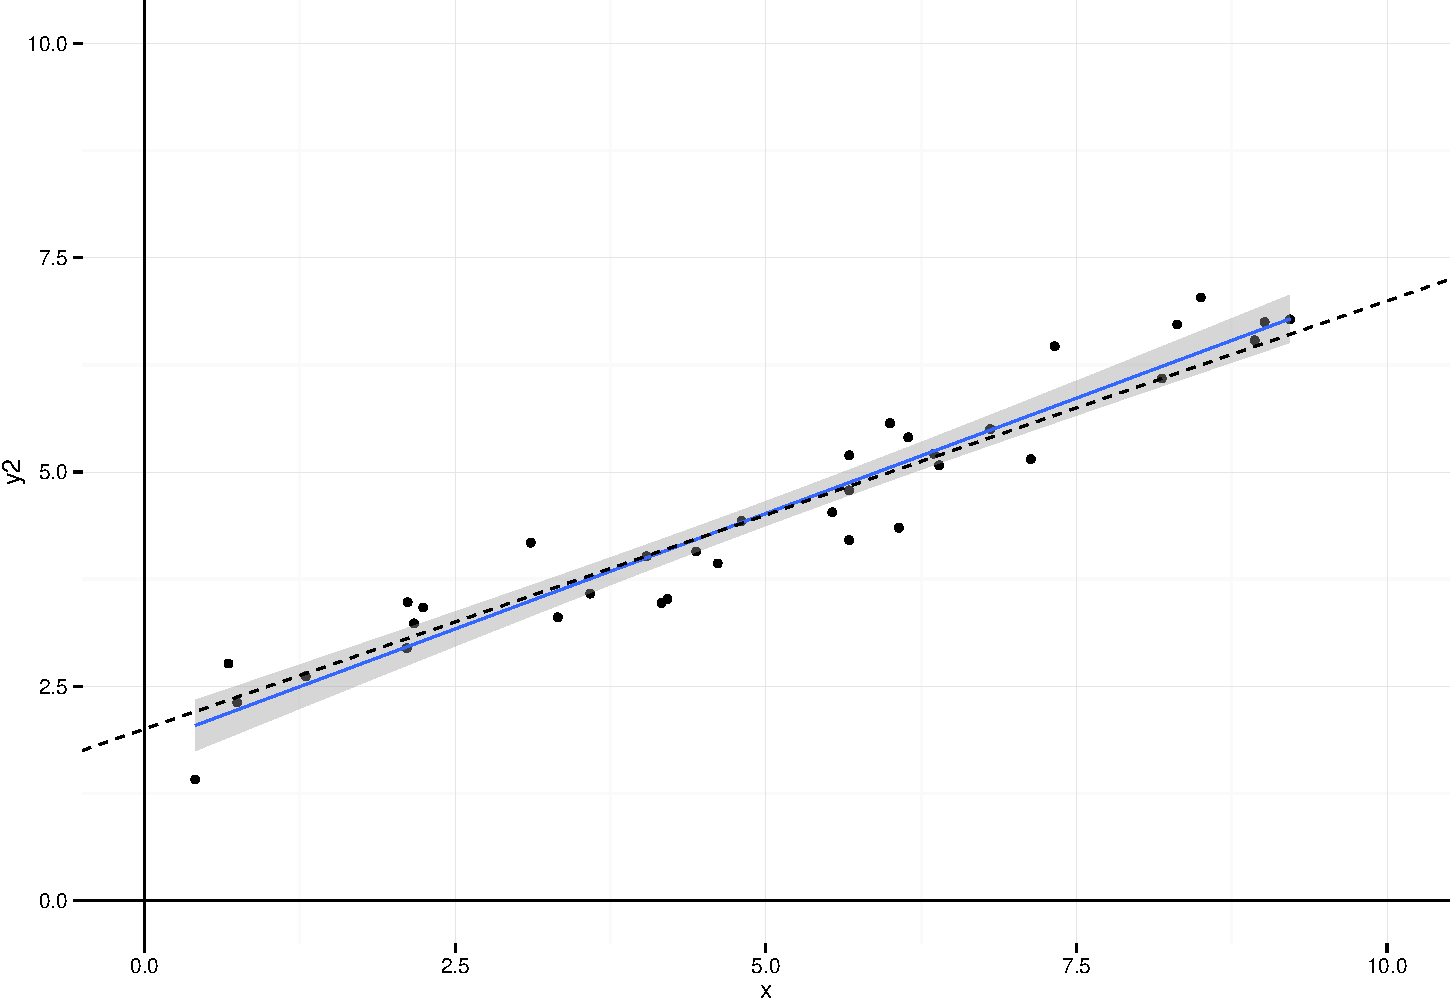
\includegraphics{Regression_files/figure-beamer/unnamed-chunk-6-1.pdf}

\end{frame}

\begin{frame}{Impact of noise}

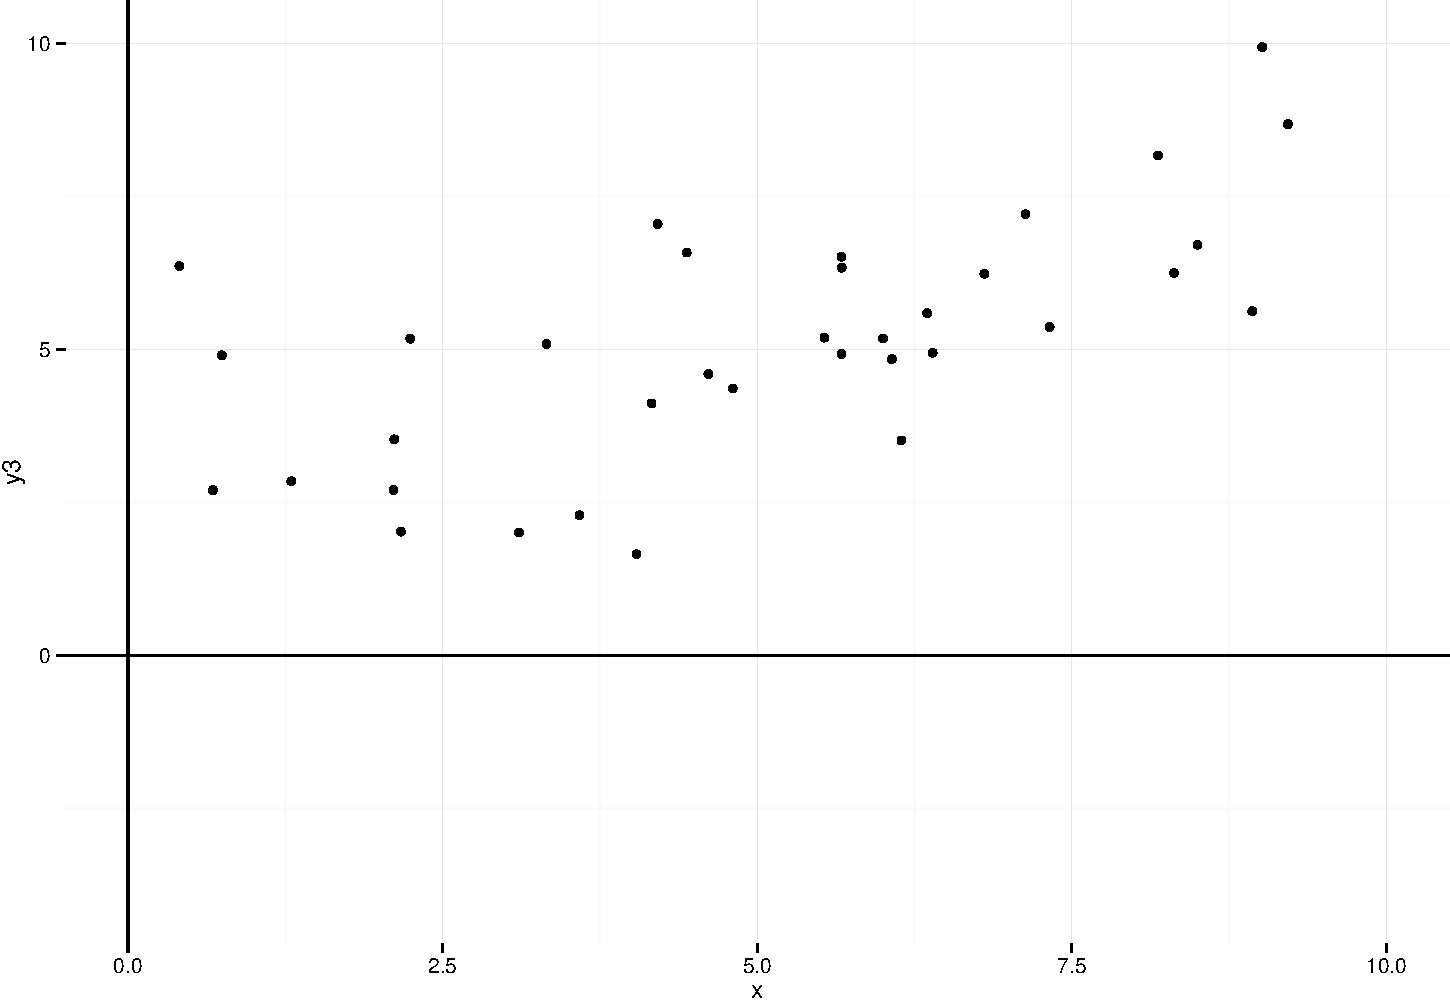
\includegraphics{Regression_files/figure-beamer/unnamed-chunk-7-1.pdf}

These data are 4 times noisier than the previous

\end{frame}

\begin{frame}{Now fit a line}

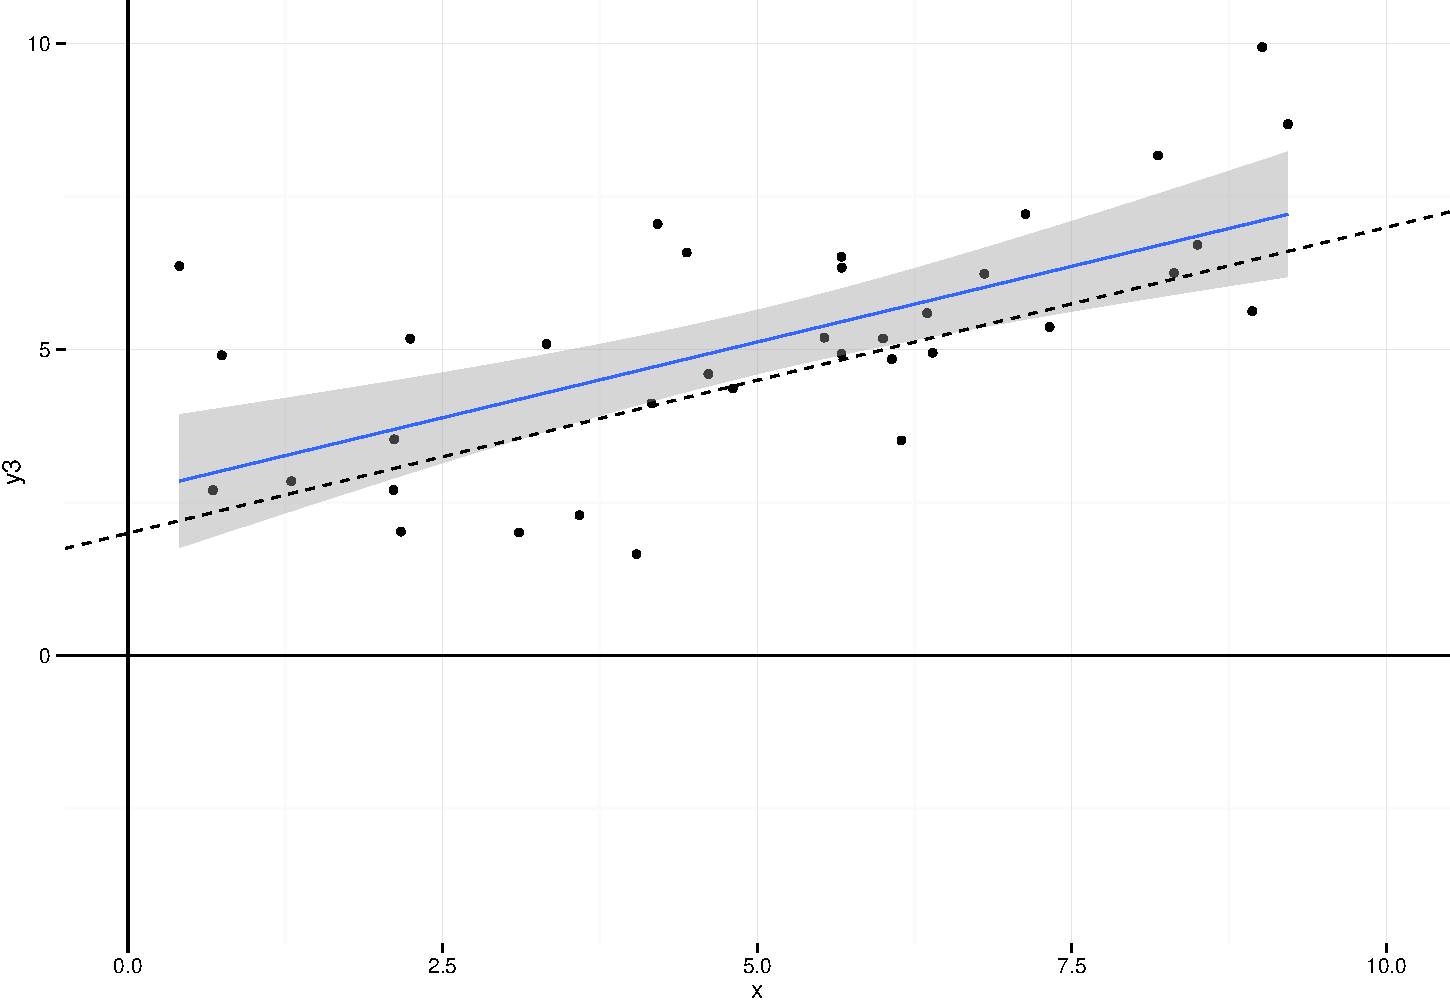
\includegraphics{Regression_files/figure-beamer/unnamed-chunk-8-1.pdf}

Dashed line is generating function.

\end{frame}


\begin{frame}[fragile]{Example: state demographics}

\begin{Shaded}
\begin{Highlighting}[]
\KeywordTok{data}\NormalTok{(state)}
\KeywordTok{kable}\NormalTok{(}\KeywordTok{head}\NormalTok{(state.x77))}
\end{Highlighting}
\end{Shaded}

\begin{longtable}[c]{@{}lrrrrrrrr@{}}
\toprule
& Population & Income & Illiteracy & Life Exp & Murder & HS Grad & Frost
& Area\tabularnewline
\midrule
\endhead
Alabama & 3615 & 3624 & 2.1 & 69.05 & 15.1 & 41.3 & 20 &
50708\tabularnewline
Alaska & 365 & 6315 & 1.5 & 69.31 & 11.3 & 66.7 & 152 &
566432\tabularnewline
Arizona & 2212 & 4530 & 1.8 & 70.55 & 7.8 & 58.1 & 15 &
113417\tabularnewline
Arkansas & 2110 & 3378 & 1.9 & 70.66 & 10.1 & 39.9 & 65 &
51945\tabularnewline
California & 21198 & 5114 & 1.1 & 71.71 & 10.3 & 62.6 & 20 &
156361\tabularnewline
Colorado & 2541 & 4884 & 0.7 & 72.06 & 6.8 & 63.9 & 166 &
103766\tabularnewline
\bottomrule
\end{longtable}

\end{frame}

\begin{frame}[fragile]{Rename the columns}

\begin{Shaded}
\begin{Highlighting}[]
\NormalTok{state =}\StringTok{ }\NormalTok{state.x77 %>%}
\StringTok{  }\KeywordTok{as.data.frame}\NormalTok{() %>%}
\StringTok{  }\KeywordTok{setNames}\NormalTok{(}\KeywordTok{c}\NormalTok{(}\StringTok{"pop"}\NormalTok{, }\StringTok{"inc"}\NormalTok{, }\StringTok{"illit"}\NormalTok{, }\StringTok{"lExp"}\NormalTok{, }\StringTok{"murder"}\NormalTok{, }\StringTok{"hsGrad"}\NormalTok{, }\StringTok{"frost"}\NormalTok{, }\StringTok{"area"}\NormalTok{))}
\KeywordTok{kable}\NormalTok{(}\KeywordTok{head}\NormalTok{(state))}
\end{Highlighting}
\end{Shaded}

\begin{longtable}[c]{@{}lrrrrrrrr@{}}
\toprule
& pop & inc & illit & lExp & murder & hsGrad & frost &
area\tabularnewline
\midrule
\endhead
Alabama & 3615 & 3624 & 2.1 & 69.05 & 15.1 & 41.3 & 20 &
50708\tabularnewline
Alaska & 365 & 6315 & 1.5 & 69.31 & 11.3 & 66.7 & 152 &
566432\tabularnewline
Arizona & 2212 & 4530 & 1.8 & 70.55 & 7.8 & 58.1 & 15 &
113417\tabularnewline
Arkansas & 2110 & 3378 & 1.9 & 70.66 & 10.1 & 39.9 & 65 &
51945\tabularnewline
California & 21198 & 5114 & 1.1 & 71.71 & 10.3 & 62.6 & 20 &
156361\tabularnewline
Colorado & 2541 & 4884 & 0.7 & 72.06 & 6.8 & 63.9 & 166 &
103766\tabularnewline
\bottomrule
\end{longtable}

\end{frame}

\begin{frame}{Inspect all pairwise relationships using \texttt{pairs()}
function}

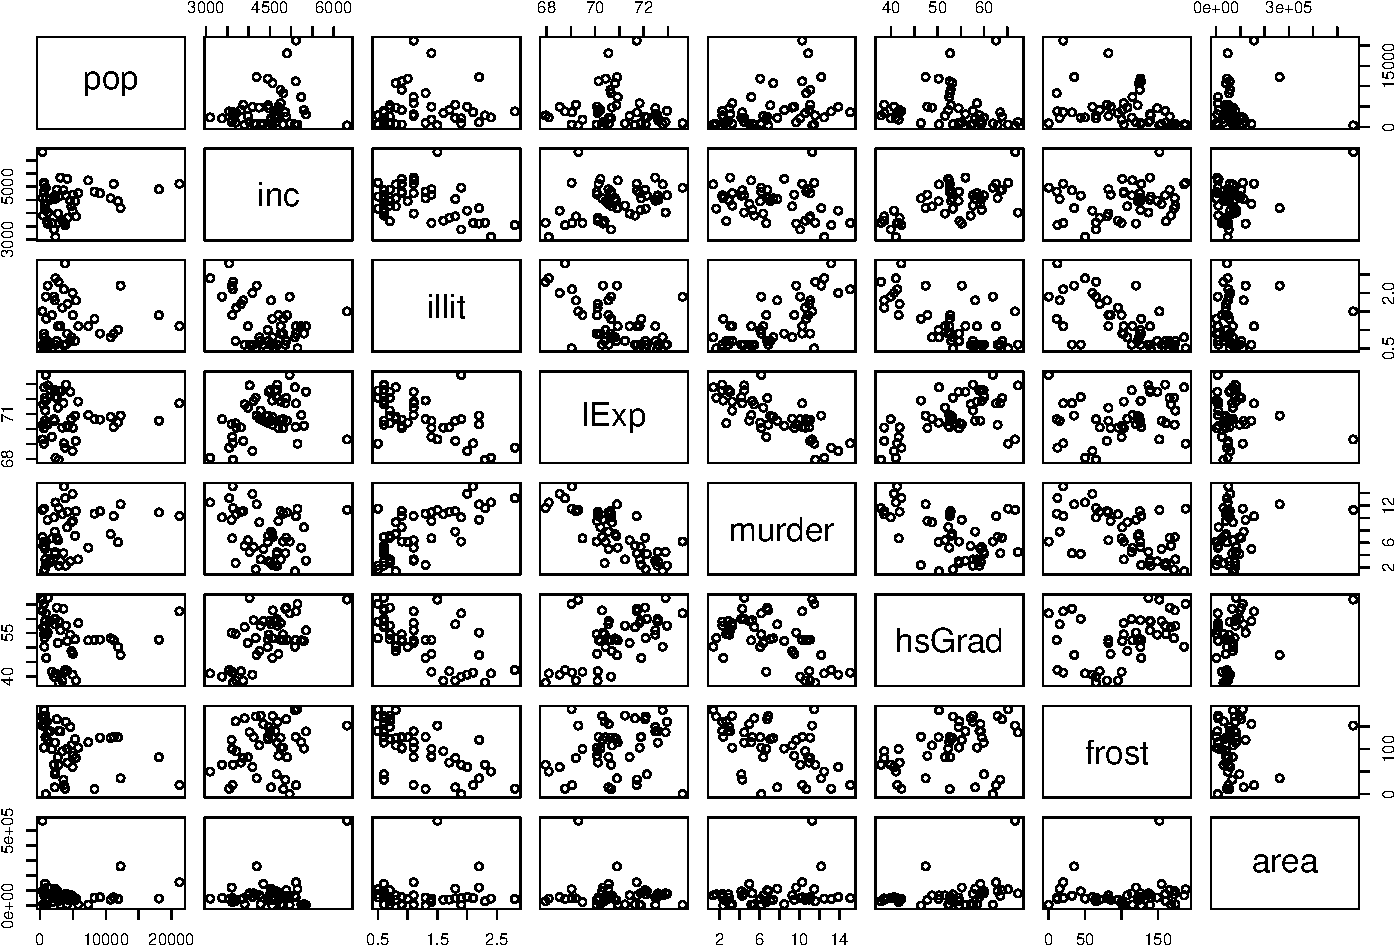
\includegraphics{Regression_files/figure-beamer/unnamed-chunk-11-1.pdf}

\end{frame}

\begin{frame}[fragile]{Make a model! For life expectancy\ldots{}}

\begin{Shaded}
\begin{Highlighting}[]
\NormalTok{mod1 =}\StringTok{ }\KeywordTok{lm}\NormalTok{(lExp ~}\StringTok{ }\NormalTok{hsGrad, state)}
\NormalTok{mod2 =}\StringTok{ }\KeywordTok{lm}\NormalTok{(lExp ~}\StringTok{ }\NormalTok{murder +}\StringTok{ }\NormalTok{hsGrad, state)}
\NormalTok{mod3 =}\StringTok{ }\KeywordTok{lm}\NormalTok{(lExp ~}\StringTok{ }\NormalTok{murder +}\StringTok{ }\NormalTok{hsGrad +}\StringTok{ }\NormalTok{illit, state)}
\end{Highlighting}
\end{Shaded}

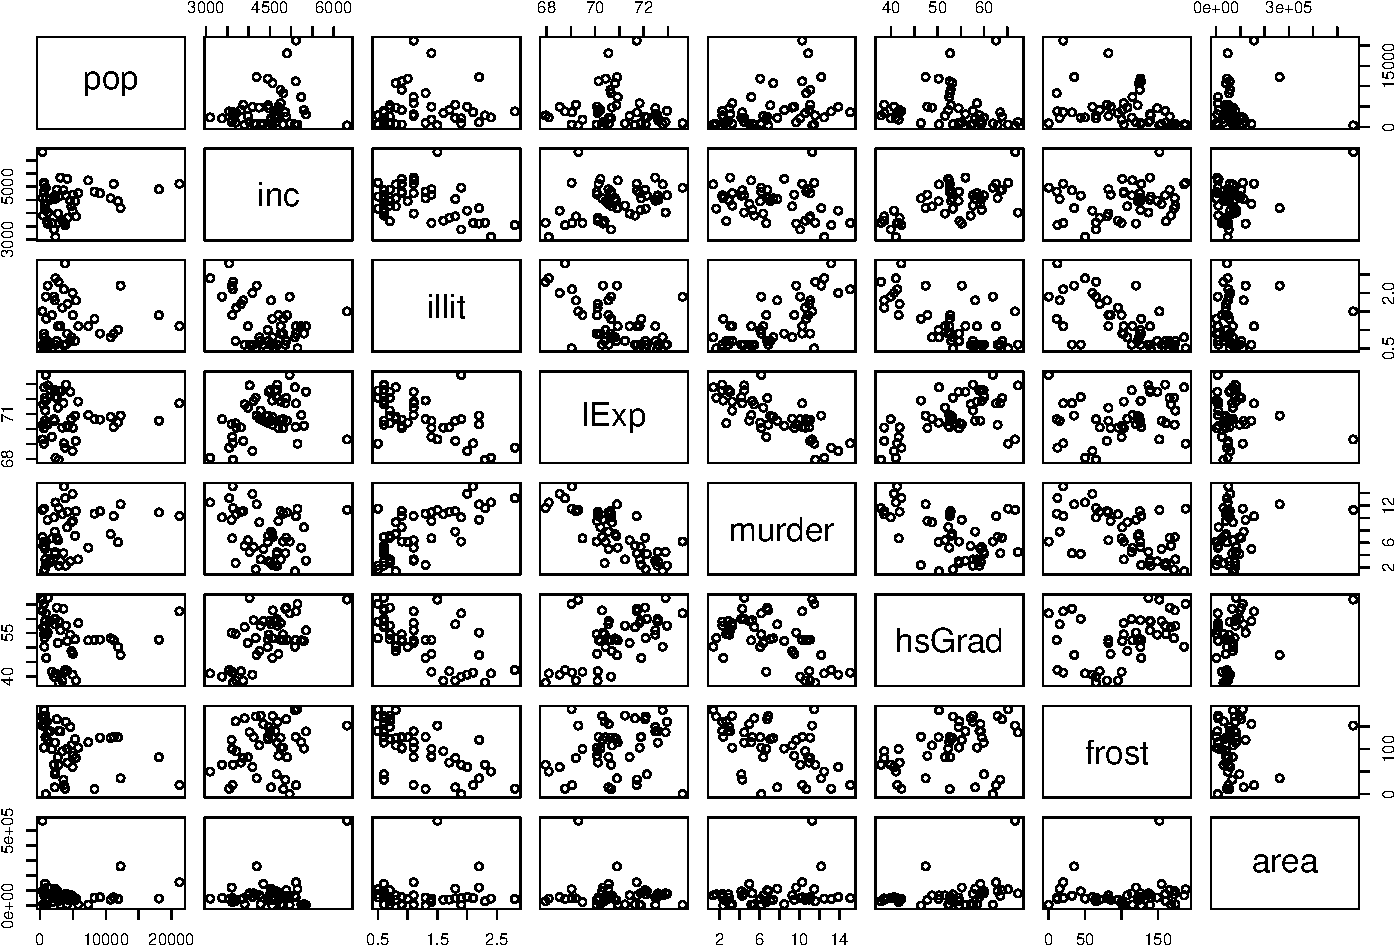
\includegraphics{Regression_files/figure-beamer/unnamed-chunk-13-1.pdf}

\end{frame}

\begin{frame}{See the good parts using \texttt{summary()}}

\end{frame}

\begin{frame}[fragile]{Model 1:}

\begin{Verbatim}[fontsize=\small]
## 
## Call:
## lm(formula = lExp ~ hsGrad, data = state)
## 
## Residuals:
##      Min       1Q   Median       3Q      Max 
## -3.01867 -0.67517 -0.07538  0.64483  2.17311 
## 
## Coefficients:
##             Estimate Std. Error t value Pr(>|t|)    
## (Intercept) 65.73965    1.04748  62.760  < 2e-16 ***
## hsGrad       0.09676    0.01950   4.961  9.2e-06 ***
## ---
## Signif. codes:  0 '***' 0.001 '**' 0.01 '*' 0.05 '.' 0.1 ' ' 1
## 
## Residual standard error: 1.103 on 48 degrees of freedom
## Multiple R-squared:  0.339,  Adjusted R-squared:  0.3252 
## F-statistic: 24.61 on 1 and 48 DF,  p-value: 9.196e-06
\end{Verbatim}

\end{frame}

\begin{frame}[fragile]{Model 2:}

\begin{Verbatim}[fontsize=\small]
## 
## Call:
## lm(formula = lExp ~ murder + hsGrad, data = state)
## 
## Residuals:
##      Min       1Q   Median       3Q      Max 
## -1.66758 -0.41801  0.05602  0.55913  2.05625 
## 
## Coefficients:
##             Estimate Std. Error t value Pr(>|t|)    
## (Intercept) 70.29708    1.01567  69.213  < 2e-16 ***
## murder      -0.23709    0.03529  -6.719 2.18e-08 ***
## hsGrad       0.04389    0.01613   2.721  0.00909 ** 
## ---
## Signif. codes:  0 '***' 0.001 '**' 0.01 '*' 0.05 '.' 0.1 ' ' 1
## 
## Residual standard error: 0.7959 on 47 degrees of freedom
## Multiple R-squared:  0.6628, Adjusted R-squared:  0.6485 
## F-statistic:  46.2 on 2 and 47 DF,  p-value: 8.016e-12
\end{Verbatim}

\end{frame}

\begin{frame}[fragile]{Model 3:}

\begin{Verbatim}[fontsize=\small]
## 
## Call:
## lm(formula = lExp ~ murder + hsGrad + illit, data = state)
## 
## Residuals:
##      Min       1Q   Median       3Q      Max 
## -1.65922 -0.46400  0.08517  0.59643  1.77657 
## 
## Coefficients:
##             Estimate Std. Error t value Pr(>|t|)    
## (Intercept) 69.73545    1.22208  57.063  < 2e-16 ***
## murder      -0.25813    0.04350  -5.934 3.63e-07 ***
## hsGrad       0.05179    0.01876   2.761  0.00825 ** 
## illit        0.25398    0.30508   0.833  0.40942    
## ---
## Signif. codes:  0 '***' 0.001 '**' 0.01 '*' 0.05 '.' 0.1 ' ' 1
## 
## Residual standard error: 0.7985 on 46 degrees of freedom
## Multiple R-squared:  0.6679, Adjusted R-squared:  0.6462 
## F-statistic: 30.83 on 3 and 46 DF,  p-value: 4.444e-11
\end{Verbatim}

\end{frame}

\begin{frame}[fragile]{Inspect the model!}

\begin{block}{\texttt{termplot()} function}

\begin{Shaded}
\begin{Highlighting}[]
\KeywordTok{par}\NormalTok{(}\DataTypeTok{mfrow =} \KeywordTok{c}\NormalTok{(}\DecValTok{1}\NormalTok{, }\DecValTok{2}\NormalTok{))}
\KeywordTok{termplot}\NormalTok{(mod2, }\DataTypeTok{partial.resid =} \OtherTok{TRUE}\NormalTok{)}
\end{Highlighting}
\end{Shaded}

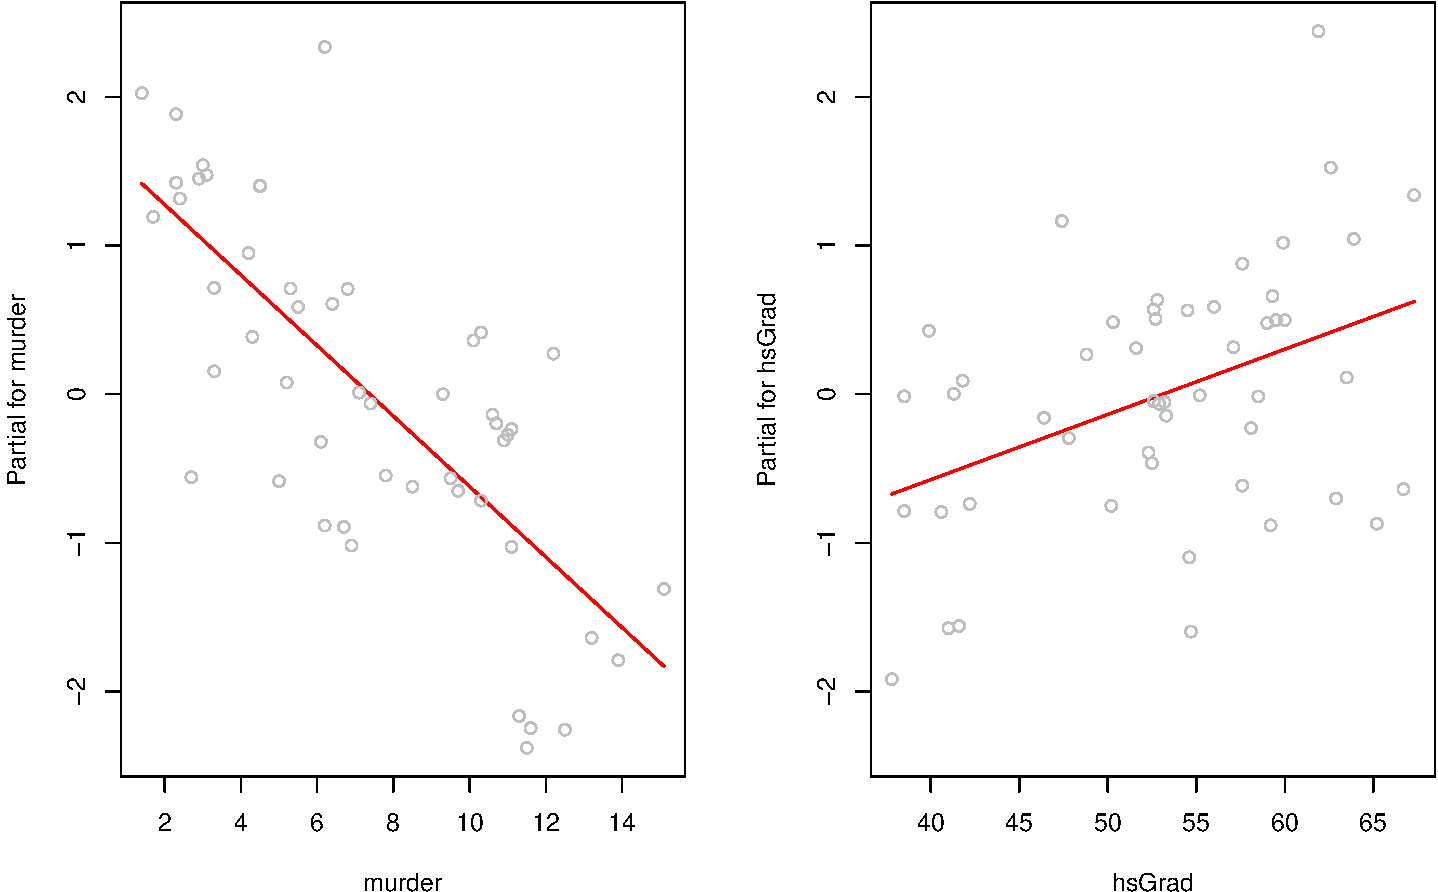
\includegraphics{Regression_files/figure-beamer/unnamed-chunk-17-1.pdf}

\begin{Shaded}
\begin{Highlighting}[]
\KeywordTok{par}\NormalTok{(}\DataTypeTok{mfrow =} \KeywordTok{c}\NormalTok{(}\DecValTok{1}\NormalTok{, }\DecValTok{1}\NormalTok{))}
\end{Highlighting}
\end{Shaded}

\end{block}

\end{frame}

\begin{frame}{\texttt{qplot()} to look at residual distribution}

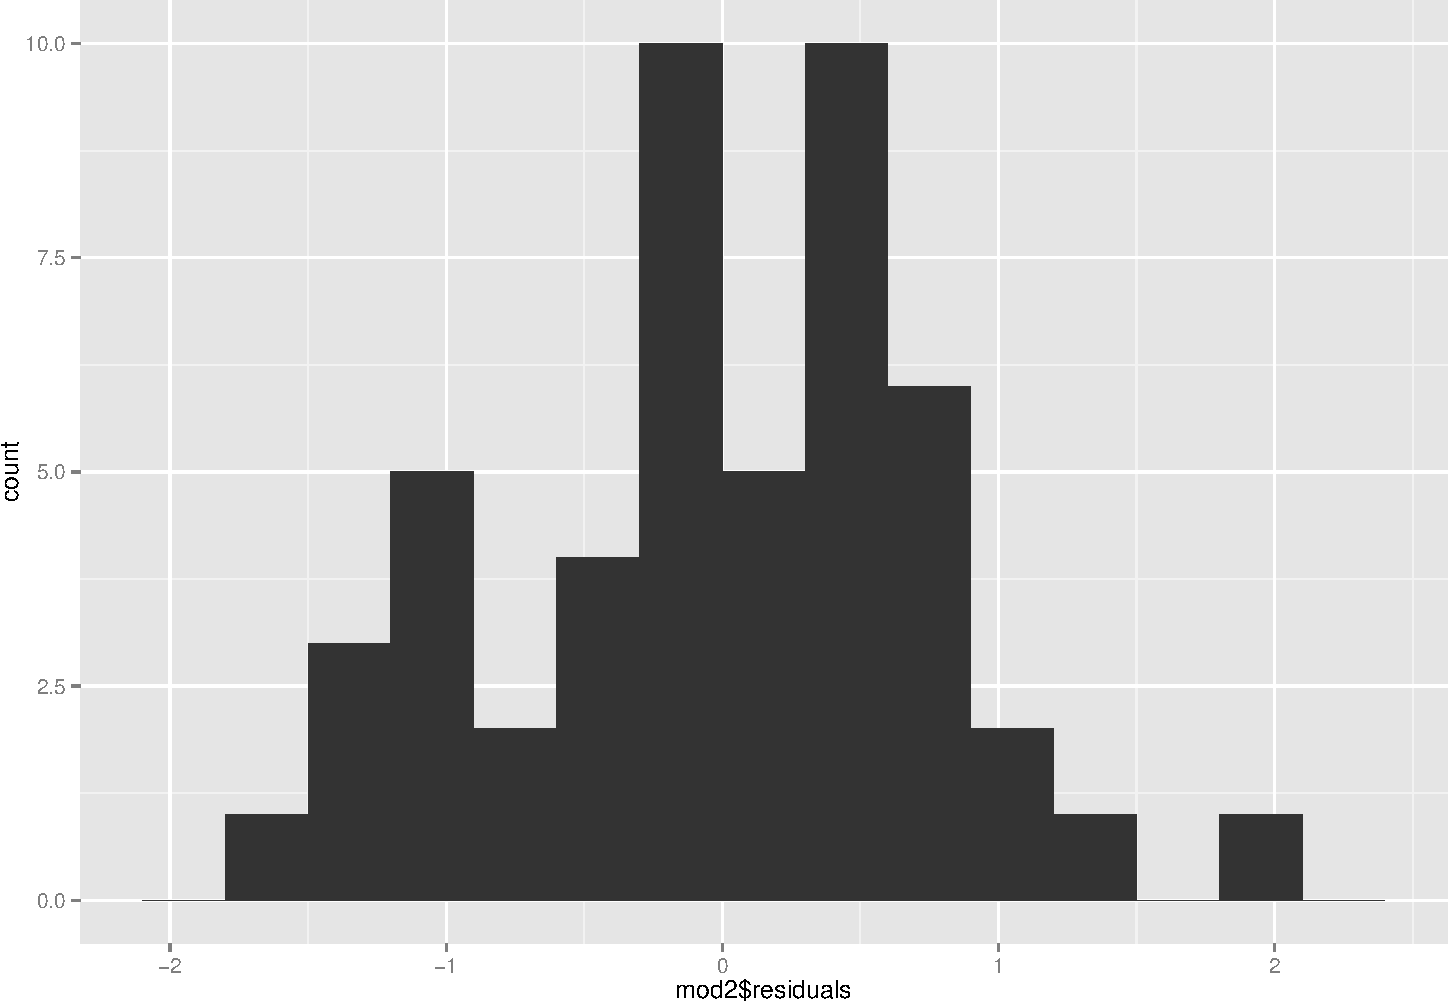
\includegraphics{Regression_files/figure-beamer/unnamed-chunk-18-1.pdf}

\begin{itemize}[<+->]
\itemsep1pt\parskip0pt\parsep0pt
\item
  Could also use \texttt{hist()}, \texttt{qqnorm()}, etc.
\end{itemize}

\end{frame}

\begin{frame}[fragile]{Make a prediction!}

\begin{block}{\texttt{predict()} function}

\begin{Shaded}
\begin{Highlighting}[]
\NormalTok{newdat =}\StringTok{ }\KeywordTok{data.frame}\NormalTok{(}\DataTypeTok{murder =} \DecValTok{9}\NormalTok{, }\DataTypeTok{hsGrad =} \DecValTok{77}\NormalTok{)}
\KeywordTok{kable}\NormalTok{(newdat)}
\end{Highlighting}
\end{Shaded}

\begin{longtable}[c]{@{}rr@{}}
\toprule
murder & hsGrad\tabularnewline
\midrule
\endhead
9 & 77\tabularnewline
\bottomrule
\end{longtable}

\end{block}

\end{frame}

\begin{frame}[fragile]{Make a prediction!}

\begin{block}{\texttt{predict()} function}

\begin{Shaded}
\begin{Highlighting}[]
\KeywordTok{predict}\NormalTok{(mod2, newdat, }\DataTypeTok{se.fit =} \OtherTok{TRUE}\NormalTok{) %>%}
\StringTok{  }\KeywordTok{as.data.frame}\NormalTok{() %>%}
\StringTok{  }\KeywordTok{kable}\NormalTok{()}
\end{Highlighting}
\end{Shaded}

\begin{longtable}[c]{@{}rrrr@{}}
\toprule
fit & se.fit & df & residual.scale\tabularnewline
\midrule
\endhead
71.5426 & 0.4311892 & 47 & 0.7958717\tabularnewline
\bottomrule
\end{longtable}

\end{block}

\end{frame}

\begin{frame}{Other topics:}

\begin{itemize}[<+->]
\itemsep1pt\parskip0pt\parsep0pt
\item
  \texttt{glm()}
\item
  \texttt{gam()} - \textbf{mgcv} package
\item
  \texttt{arima()} - time series models
\item
  automated model selection

  \begin{itemize}[<+->]
  \itemsep1pt\parskip0pt\parsep0pt
  \item
    stepwise \texttt{step()} function,
  \item
    best subset \textbf{leaps} package
  \end{itemize}
\item
  machine learning methods - various packages
\end{itemize}

That's all!

\end{frame}

\end{document}
